\documentclass[printbox]{BHCexam}
\biaoti{~$2013 - 2014$~学年度第一学期期末考试}
\fubiaoti{高三数学试卷}
\usepackage{palatino}
\usepackage{siunitx}%输入度数符号需要的单位宏包
\usepackage{tikz}
\usetikzlibrary{shapes.geometric, arrows}
\tikzstyle{startstop} = [rectangle, rounded corners, minimum width = 1cm, minimum height=0.5cm,text centered, draw = black]
\tikzstyle{io} = [trapezium, trapezium left angle=70, trapezium right angle=110, minimum width=0.5cm, minimum height=0.5cm, text centered, draw=black]
\tikzstyle{process} = [rectangle, minimum width=2cm, minimum height=0.5cm, text centered, draw=black]
\tikzstyle{decision} = [diamond, aspect = 3, text centered, draw=black]
% 箭头形式
\tikzstyle{arrow} = [->,>=latex]
\begin{document}
\maketitle
%\mininotice
\notice
\begin{questions}

%选择题
\xuanze
\question 已知集合~$A=\{ -1,0,1 \},B=\{ x|-1\leq x<1 \}$~,则~$A\cap B=$~\xx.
\onech{$\{0 \}$}{$\{-1,0 \}$}{$\{0,1 \}$}{$\{-1,0,1 \}$}
\question 复数~$z=\dfrac{(1-i)^2}{1+i}$(~$i$~为虚数单位)~的虚部为\xx.
\onech{$1$}{$0$}{$\pm 1$}{$-1$}
\question 已知椭圆~$\dfrac{x^2}{16}+\dfrac{y^2}{m}=1$~的一个焦点为~$F(3,0)$~,则~$m=$~\xx.
\onech{$3$}{$7$}{$9$}{$25$}
\question 下列函数中,既是奇函数又是定义域上的增函数的是\xx.
\onech{$y=2x+1$}{$y=e^x-e^{-x}$}{$y=\dfrac{-2}{x}$}{$y=x\sqrt{x}$}
\question 设等差数列~$\{a_n \}$~的前~$n$~项和为~$S_n$~,若~$S_3=18$~,则~$a_2$~\xx.
\onech{$7$}{$5$}{$6$}{$4$}
\begin{minipage}[b]{0.6\linewidth}
\question 函数~$f(x)=A\sin (\omega x+\varphi)$($A,\omega,\varphi$~是常数,~$A>0,\omega >0$)~的部分图象如图所示,则函数~$f(x)$~的单调增区间可能为\xx.
\fourch{$\left[ -\dfrac{5\pi}{12},\dfrac{\pi}{12} \right]$}{$\left[ -\dfrac{\pi}{3},\dfrac{\pi}{6} \right]$}%
{$\left[ \dfrac{\pi}{12},\dfrac{7\pi}{12} \right]$}{$\left[ -\dfrac{\pi}{12},\dfrac{5\pi}{12} \right]$}
\question 执行如图所示的程序框图,输出的$s$值为~\xx.
\fourch{$-3$}{$-\dfrac{1}{2}$}{$2$}{$\dfrac{1}{3}$}
\end{minipage}
\begin{minipage}[b]{0.4\linewidth}
\begin{flushright}
\begin{tikzpicture}[scale=0.8]
\coordinate[label=below right:\small $O$] (O) at(0,0);
\coordinate[label=above :\small $\dfrac{\pi}{3}$] (t1) at(pi/3,0);
\coordinate[label=above :\small $\dfrac{7\pi}{12}$] (t2) at(7*pi/12,0);
\draw[->,>=latex](-pi/2,0)--(pi,0)node[below](x) {$x$};
\draw[->,>=latex](0,-1.5)--(0,1.5)node[right](y) {\small $y$};
\draw [domain=-pi/6:5*pi/6,samples=1000] plot(\x,{sin((2*(\x)+pi/3) r)});
\draw[densely dashed](0,-1)--(7*pi/12,-1)--(7*pi/12,0);
\node[left](pi) at(0,-1) {\small $-2$};
\end{tikzpicture}
\begin{tikzpicture}[node distance=0.2cm][scale=0.4]
%定义流程图具体形状
\node[startstop](start){开始};
\node[process, below of = start, yshift = -1cm](in1){$i=0,s=2$};
%\node[process, below of = in1, yshift = -1cm](pro1){$S=\frac{1}{1-S}$};
%\node[decision, below of = pro1, yshift = -1cm](dec1){Decision 1 ?};
%\node[process, below of = pro1, yshift = -1cm](pro2){$n=n+1$};
\node[decision, below of = in1, yshift = -2.5cm](dec1){$i<4$};
\node[process, right of = dec1, xshift = 2.5cm](pro2){$i=i+1$};
\node[process, above of = pro2, yshift = 1cm](pro3){$s= \frac{s-1}{s+1}$};
\node[io, below of = dec1, yshift = -1cm](out1){输出~$s$~};
\node[startstop, below of = out1, yshift = -1cm](stop){结束};
%\coordinate (point1) at (-1cm, -4cm);
%连接具体形状
\draw [arrow] (start) -- (in1);
\draw [arrow] (in1) -- (dec1);
\draw [arrow] (dec1) --node [right] {否} (out1);
\draw [arrow](dec1) -- node [above] {是} (pro2);
\draw [arrow] (pro2) -- (pro3);
%\draw [arrow] (dec1) -- node [left] {否} (pro1);
%\draw [arrow] (dec1) -- node [right] {是} (out1);
\draw [arrow] (out1) -- (stop);
\draw [arrow] (2.7,-2.36) -- (2.7,-2) -- (0,-2);
\end{tikzpicture}
\end{flushright}
\end{minipage}
\question 下列有关命题的说法正确的是\xx.
\fourch{命题“若~$x=y$~,则~$\sin x=\sin y$~”的逆否命题为真命题}{函数~$f(x)=\tan x$~的定义域为~$\{x\,|\,x\neq k\pi,k\in Z$~}
{命题“~$\exists x\in R$~使得~$x^2+x+1<0$~”的否定是:“~$\forall x\in R$~,均有~$x^2+x+1<0$~".}
{“$a=2$~”是“直线~$y=-ax+2$~与~$y=\dfrac{a}{x} x-1$~垂直”的必要不充分条件.}
\begin{minipage}[b]{0.6\linewidth}
\question 设函数~$y=x^3$~与~$y=\left(\dfrac{1}{2} \right)^{x-2}$~的图象的交点为~$(~x_0,y_0~)$~,则~$x_0$~所在的区间是\xx.
\twoch{$(0,1)$}{$(1,2)$}{$(2,3)$}{$(3,4)$}
\question 一个空间几何体的三视图如图,则该几何体的体积为\xx.
\twoch{$2\sqrt{3}$}{$2\sqrt{5}$}{$\dfrac{4\sqrt{3}}{3}$}{$\dfrac{5\sqrt{3}}{3}$}
\end{minipage}
%\hfill
\begin{minipage}[b]{0.4\linewidth}
\begin{flushright}
\begin{tikzpicture}[scale=0.9]
\tikzmath{
\a=sqrt(2);
\b=\a/2;
}
\coordinate (p) at (0,0) {};
%\draw (p)--++(-1,0)--++(2,0)--++(-1,0)--cycle;
\draw (p) rectangle +(2,2);
\coordinate(o) at (1,1) {};
\draw (0,2)--(o)--(2,2) (o)--(1,0);
%\draw[densely dashed,thin] (p)--($(p)+(2,2)$);
%\draw ($(p)$)--($(p)+(1,0)$)--($(p)+(2,0)$);
\node (p1) at (0.5,-0.2) {\tiny 1};
\draw[->|,>=stealth](p1)--($(p1)+(0.5,0)$);
\draw[->|,>=stealth](p1)--($(p1)+(-0.5,0)$);
\node (p2) at (1.5,-0.2){\tiny 1};
\draw[->|,>=stealth](p2)--($(p2)+(0.5,0)$);
\draw[->|,>=stealth](p2)--($(p2)+(-0.5,0)$);
\node (p3) at (2.2,0.5) {\tiny 1};
\draw[->|,>=stealth](p3)--($(p3)+(0,0.5)$);
\draw[->|,>=stealth](p3)--($(p3)+(0,-0.5)$);
\node (p4) at (2.2,1.5) {\tiny 1};
\draw[->|,>=stealth](p4)--($(p4)+(0,0.5)$);
\draw[->|,>=stealth](p4)--($(p4)+(0,-0.5)$);
\node (s) at(1,-0.5){\small 正视图}; 
\begin{scope}[xshift=2.5 cm]
\coordinate (p) at (0,0);
\draw (p)--+($(\a,0)$)--+($(\a,\a)$)--+($(0,2)$)--cycle;
\node(p2) at (\b,-0.2){\tiny $\sqrt{3}$};
\draw [->|,>=stealth](p2)--($(p2)+(0.7,0)$);
\draw [->|,>=stealth](p2)--($(p2)+(-0.7,0)$);
\node (s) at(\b,-0.5){\small 侧视图}; 
\end{scope}
\begin{scope}[yshift=-1cm]
\draw (0,0)--+(2,0)--+(1,-1.5)--cycle;
\node (s) at(1,-1.8){\small 俯视图}; 
%\caption{俯视图}
\end{scope}
\end{tikzpicture}
\end{flushright}
\end{minipage}

%填空题
\tiankong
\question 已知向量~$\vec{a}=(3,1),\vec{b}=(1,3),\vec{c}=(k,7)$~,若~$(\vec{a}-\vec{c}) \parallel \vec{b}$~,则~$k=$~\mtk{}.
\question 等比数列~$\{a_n \}$~的公比~$q>0$~,已知~$a_2=1,a_{n+2}+a_{n+1}=6a_n$~,则~$\{a_n \}$~的前~$4$~项和~$S_4$~\mtk{}.
\question 设~$z=kx+y$~,其中实数~$x,y$~满足~$ \begin{cases}
x+y-2\geq 0,\\
x-2y+4\geq 0, \\
2x-y-4\leq 0,
\end{cases}$若~$z$~的最大值为~$12$~,则实数~$k=$~\mtk{}.
\question 设~$f(x)$~表示~$x+2$~与~$x^2+3x+2$~中的较大者,则~$f(x)$~的最小值为\mtk{}.
\question 设~$a\in R,f(x)=\cos (a\sin x-\cos x)+\sin ^2 x$~的定义域是~$\left[ \dfrac{\pi}{4},\dfrac{11}{24} \pi \right]~,f(\dfrac{\pi}{4})=\sqrt{3}$~.\\给出下列几个命题:\\
\ding{192}~$f(x)$~在~$x=\dfrac{\pi}{4}$~处取得最小值;\ding{193}~$\left[ \dfrac{5}{12} \pi,\dfrac{11}{24} \pi \right]$~是~$f(x)$~的一个单调递减区间;\\
\ding{194}~$f(x)$~的图象向左平移~$\dfrac{\pi}{12}$~个单位,将得到函数~$y=2\sin {2x}$~的图象;\\
\ding{195}使得~$f(x)$~取得最大值的点仅有一个~$x=\dfrac{\pi}{3}$~.\\
其中正确命题的序号是\mtk{}.(将你认为正确命题的序号都填上)
%解答题
\jianda
\question 在~$\triangle ABC$~中,角~$A,B,C$~的对边分别为~$a,b,c$~,已知~$A=\dfrac{\pi}{2}+C,\sin (A+C)=\dfrac{3}{5}$~.
\begin{parts}
\part 求~$\cos C$~的值;
\part 若~$a+c=3\sqrt{5}$~,求~$\triangle ABC$~的面积.
\end{parts}
\question 有甲乙两个班级进行数学考试,按照大于等于分为优秀,分以下为非优秀统计成绩后,得到如下的列联表.
\begin{center}
\begin{tabular}{|c|c|c|c|}
\hline
~~~~~~~{}~~~~~~~&~~~~~~~优秀~~~~~~~&~~~~~~~非优秀~~~~~~~&~~~~~~~总计~~~~~~~\\
\hline
~~~~~~~甲班~~~~~~~&~~~~~~~10~~~~~~~&~~~~~~~{}~~~~~~~&~~~~~~~{}~~~~~~~\\
\hline
~~~~~~~乙班~~~~~~~&~~~~~~~{}~~~~~~~&~~~~~~~30~~~~~~~&~~~~~~~{}~~~~~~~\\
\hline
~~~~~~~合计~~~~~~~&~~~~~~~{}~~~~~~~&~~~~~~~{}~~~~~~~&~~~~~~~105~~~~~~~\\
\hline
\end{tabular}
\end{center}
已知在全部~$105$~人中抽到随机抽取~$1$~人为优秀的概率为~$\dfrac{2}{7}$~.
\begin{parts}
\part 请完成上面的列联表; 
\part 根据列联表的数据,若按~$95 \%$~的可靠性要求,能否认为”成绩与班级有关系”;
\part 若按下面的方法从甲班优秀的学生抽取一人:把甲班优秀的~$10$~名学生从~$2$~到~$11$~进行编号,先后两次抛掷一枚均匀的骰子,出现的点数之和为被抽取人的序号.试求抽到~$6$~或~$11$~号的概率.
\end{parts}
下面临界值表仅参考:
\begin{tabular}{|c|c|c|c|c|c|c|c|}
\hline
$P(K^2\geq k_0)$&$0.15$&$0.10$&$0.05$&$0.025$&$0.010$&$0.005$&$0.001$\\
\hline
$k_0$&$2.072$&$2.706$&$3.841$&$5.024$&$6.635$&$7.879$&$10.828$\\
\hline
\end{tabular}\\
(参考公式:~$K^2=\dfrac{n(ad-bc)^2}{(a+b)(c+d)(a+c)(b+d)}$~,其中~$n=a+b+c+d$~)
\vspace{6cm}
\question 已知数列~$\{a_n \}$~是公差不为~$0$~的等差数列,~$a_1=2$~且~$a_2,a_3,a_4+1$~成等比数列.
\begin{parts}
\part 求数列~$\{a_n \}$~的通项公式;
\part 设~$b_n=\dfrac{2}{n\cdot (a_n+2)}$~,求数列~$\{b_n \}$~的前~$n$~项和~$S_n$~.
\end{parts}

\question 如图,在直三棱柱~$ABC--A_1B_1C_1$~中,~$AA_1=2,AB=AC=1,\angle BAC=90^{\circ}$~,点~$M$~是~$BC$~的中点,点~$N$~在侧棱~$CC_1$~上.
\begin{parts}
\part 求证:~$A_1C \parallel$~ 面~$AB_1M$~;
\part 当线段~$CN$~的长度为多少时,~$NM\perp AB_1$~.
\end{parts}
\begin{flushright}
\begin{tikzpicture}
\coordinate[label=below left:$B$](B) at (0,0);
\coordinate[label=below right:$C$](C) at (3,0);
\coordinate[label=left:$B_1$](B_1) at (0,3);
\coordinate[label=right:$C_1$](C_1) at (3,3);
\draw(B)--(C)--(C_1)--(B_1)--cycle;
\coordinate[label=above right:$A$](A) at (1.6,0.866);
\coordinate[label=above:$A_1$](A_1) at (1.6,3.866);
\coordinate[label=below:$M$](M) at ($(B)!0.5!(C)$);
\coordinate[label=right:$N$](N) at ($(C)!0.4!(C_1)$);
\draw(B_1)--(M)--(N)--(B_1);
\draw(B)--(A)--(C);
\draw(B_1)--(A_1)--(C_1);
\draw[dashed] (B)--(A_1)--(C) (B_1)--(A) (A)--(M) (A)--(N) (A)--(A_1);
\end{tikzpicture}
\end{flushright}
\vspace{3cm}
\question 已知~$E(2,2)$~是抛物线~$C:y^2=2px(p>0)$~上一点,经过点~$(2,0)$~的直线~$l$~与抛物线~$C$~交于~$A,B$~两点(不同于点~$E$~),直线~$EA,EB$~分别交直线~$x=-2$~于点~$M,N$~.
\begin{parts}
\part 求抛物线方程及其焦点坐标;
\part 已知~$O$~为原点,求证:~$\overrightarrow{OM}\cdot \overrightarrow{ON}=0$~
\end{parts}
\vspace{6cm}
\question 已知函数~$f(x)=x-a\ln x,g(x)=\dfrac{1+a}{x}(a\in R)$~.
\begin{parts}
\part 当~$a=1$~时,求曲线~$f(x)$~在~$x=1$~处的切线方程;
\part 设函数~$h(x)=f(x)-g(x)$~,求函数~$h(x)$~的单调区间.
\end{parts}
\end{questions}
\end{document}
